\documentclass[10pt]{article}
\usepackage[top = 1in,
            left = 1in,
            right = 1in,
            bottom = 1in]{geometry}
\usepackage{amsmath}
\usepackage{stackengine}
\usepackage{amsfonts}
\usepackage{minted}
\usepackage{graphicx}
\newcounter{counter}
\setcounter{counter}{1}
\newcommand*{\lo}[1]{
    \textbf{* #1} \newline
}
\newcommand*{\question}[1]{
            \textbf{\thecounter. #1} \hfill
            \addtocounter{counter}{1}
            
            \newblock

            }
\setlength\parindent{0pt}
\begin{document}
\begin{center}
    \section*{EECS 334 Final Review}
\end{center}
\question{Compute the resultant irradiance of coherent and incoherent superposition of waves of the same frequency.}
Lets define coherent waves; two waves sources are coherent if their \textbf{frequency} and \textbf{waveform} are identical.
\begin{center}
    \includegraphics*[scale = 1]{imgs/coherent-wave.png}    
\end{center}

Lastly, the definition of incoherent waves is two or more waves that have don't have the same frequency and phase.

\begin{center}
    \includegraphics*[scale = .5]{imgs/phase-difference.png}
\end{center}

\newpage 

So, what this statement is asking us is to add these two waves, which we can do because of superposition! Superposition is the fact that if we have $\lambda_1$ and $\lambda_2$ we can add them together. If they interfere \textbf{constructively} then they will add into a bigger wave than the original, if interfere \textbf{destructive}, then the resulting wave is smaller.

\begin{center}
    \includegraphics*[scale = .5]{imgs/superposition.png}
\end{center}
We can say that the resulting wave due to the two path differences is
\[E_R = E_1 + E_2 = E_{01}\cos(\alpha_1 - wt) + E_{02}\cos(\alpha_2 - wt)\]
\begin{itemize}
    \item If $(\alpha_2 - \alpha_1) = m2\pi$, where $m$ is an integer, then the waves are in-step (the peaks and the troughs arrive at a point $P$ at the same time). This is \textbf{constructive interference}.
    \item $(\alpha_2 - \alpha_1) = (2m+1)\pi$, then the waves are out of step, resulting in \textbf{destructive interference}.
\end{itemize}

\textit{Note: When you hear out of phase, it usually means the wave source is shifted by $\pi$.}

\newblock

A real life example of destructive interference. When someone is wearing noise cancelling headphones, the noise coming in has its own wave, but the headphones will send a single back cancelling out the the original wave. This is using the idea of two waves being completely destructive!
\begin{center}
    \includegraphics*[scale = .25]{imgs/wavelength-fact.jpeg}
\end{center}

\newpage

If we keep shifting to the right by an integer value, we will keep on getting constructive interference! Look at the diagram below. Wavelength 2 is red and wavelength 1 is black.

\begin{center}
    \includegraphics*[scale = .35]{imgs/interger-difference.jpeg}
\end{center}

Now let's try an example.\\ \\
\textbf{Example:} \\ \\ 
Determine the result of the superposition of the following harmonic waves:
\textit{Note: $\frac{\pi}{3}$ is the phase shift, $\omega$ is the frequency.}
\[E_1 = 7 \cos(\frac{\pi}{3} - \omega t), E_2 = 12 \sin(\frac{\pi}{4} - \omega t), \text{, and } E_3 = 20 \cos(\frac{\pi}{5} - \omega t)\]

The first thing we need to do is make all the phase angles consistent. We do this by making them all the same trig function.

\begin{center}
    \includegraphics*[scale = .2]{imgs/superposition-example.jpeg}
\end{center}

Now that we have the amplitude, lets het the phase angle. We can achieve this by 
\[\tan(\alpha) = \frac{9.33}{28.165},\qquad \alpha = 0.32\text{rad}\]

Therefore, the resulting wave is 

\[\boxed{E_R = 29.67 \cos(0.32 - \omega t)} \]

\textit{Note: We "got rid" of $\omega$ and $t$ from the calculations because we are taking a screen shot of the waves and finding their superposition.}

\newblock

Now, let's talk about \textbf{Random} and \textbf{Coherent sources}. For $N$ randomly phased (meaning $\varphi$) of equal amplitude and frequency we can find the irradiance by using 
\[E_0^2 = N\cdot E_0^2\]

Let's say the $N$ sources are coherent (peaks and troughs match) and in-phase so that all $\alpha_i$ are equal and amplitudes are equal, then we can find irradiance by 

\[E_0^2 = N^2 \cdot E_0^2\]

\newblock

\question{Explain the properties of standing waves and of the modes of a cavity}

The definition of a \textbf{standing wave} is when we confine a wave in a medium that has boundaries, and then this wave will reflect at the boundary, and the wave will overlap with itself. 

\newblock

The reason why we care about these \textbf{standing waves} is that they select preferred wavelengths ($\lambda$), and frequency $\omega$, and this wave becomes dominant in the medium. 

\newblock

Lets think of a an example, when we pluck a guitar string it oscillates, and this is true for waves! So, when we plunk this string it will hit the end of a medium, lets call this a node, and when the wave reaches the node it will reflect back on itself.

\begin{center}
    \includegraphics*[scale = .2]{imgs/standing-wave-diagram.jpeg}
\end{center}

Now, lets analyze what this would be if we have a wavelength inside of this cavity. We see that we have destructive interference at these nodes, and we have constructive interference between these nodes.

\begin{center}
    \includegraphics*[scale = .15]{imgs/standing-wave-with-nodes.jpeg}
\end{center}

\newpage

\begin{center}
    \includegraphics*[scale = .75]{imgs/book-standing-wave-diagram.png}
\end{center}

Above is a diagram pulled from the book to show us the equation of the resulting \textbf{standing wave}. We see that \textbf{constructive interference} happens at $t = \frac{T}{2}, \frac{3T}{2}, \dots$, and we get \textbf{destructive interference} at $t = 0, T, 2T, \dots$ \textit{Note: $\varphi_R$ is a phase shift of $\pi$ upon reflection. Also, where constructive interference happens, this is called an anti-node.}

\newblock

Let's say that the phase shift due to reflection ($\varphi_R$) is not equal to $\pi$, then the node position is shift, but the nodes are still separated by half of a wavelength ($\frac{\lambda}{2}$), and the anti-nodes are shifted too! This is still a standing wave.

\newblock

An important idea behind \textbf{standing waves} is that they transmit no energy, unlike traveling waves. Another example of standing waves are lasers! Lasers use standing waves, by forming a cavity between two mirrors to send a wave back and forth like the image below.

\begin{center}
    \includegraphics*[scale = .75]{imgs/standing-wave-for-lazer.png}
\end{center}

Looking at the diagram above we see that only wavelengths with descrete values like a inteeger number of half-wavelengths will fit into the distance between the two mirrors, which we will label $d$.

\[d = m \bigg( \frac{\lambda\cdot m}{2} \bigg)\]

\newpage

We can also find the the wavelength of the standing wave modes by: 

\[\lambda_m = \frac{2d}{m}\]

Also, we can find the frequencies of the standing wave modes ($\nu_m$):

\[\nu_m = \frac{v}{\lambda} \to \text{ we know that the wave is light so $v = c$, so}\]
\[ \nu_m = \frac{v}{\lambda} = \frac{c}{\lambda} = \frac{c\cdot m}{2d}\]

Note that these equations are only valid for cavities with plane mirrors.

\textbf{Example} 
\\ \newblock
A certain He-Ne laser cavity of the type shown in Figure 6 has a mirror
separation of 30 cm. The helium-neon laser gain medium is capable of
supporting laser light of wavelengths in the range from $\lambda_1 = 632.8$nm to $\lambda_2 = 632.802$nm, find:
\\ \newblock
a. The approximate number $m$ of half-wavelengths that fit into the cavity

b. The range of frequencies supported by the helium-neon gain medium

c. The difference in the frequencies of adjacent standing wave modes of
the cavity

d. The number of standing wave modes that will likely be present in the
laser output

\begin{center}
    \includegraphics*[scale = .2]{imgs/cavity-example.jpeg}
\end{center}

\newpage

\begin{center}
    \includegraphics*[scale = .2]{imgs/cavity-example-cont.jpeg}
\end{center}
\textbf{LEARNING OUTCOMES:} \\ 
\fbox
{
    \begin{minipage}{\linewidth}
    1. Forward and a reverse wave exist, which will take on the following form of
    \[E_R = A(x)\cos(\omega t)\]
    where $A(x)$ is the amplitude and $\omega$ is the frequency.

    \newblock

    2. The equation for a standing wave is 
    \[2E_0 \sin(kx)\]

    3. Nodes where $A(x) = 0$ or at $x = m (\frac{\lambda}{2})$
    \end{minipage}
}

\newpage

\question{Determine the beat frequency of two waves.}

\textbf{Beat Frequency} is when we have two waves of different frequency ($\omega$) and wavelength ($\lambda$), and find the difference between their frequencies:

\[\omega_b = 2 \cdot \omega_g = 2 \frac{(\omega_2 - \omega_1)}{2} = \omega_2 - \omega_1\]

\begin{center}
    \includegraphics*[scale = .25]{imgs/book-example-beat-frequency.png}
\end{center}
We can see that the resulting wave makes this odd wave. Beat frequency looks like it starts of constructive, and then it will become destructive with the other wave, and it will oscillate between these two stages. (Also, this leads to pulses of energy!)

\newblock

\textbf{LEARNING OUTCOMES:} \\ 
\fbox
{
    \begin{minipage}{\linewidth}
        
    
    1. Lets say we have two wavelengths $E_1$ and $E_2$ where
    \[E_1 = E_0\cos(k_1x - \omega t) \qquad E_2 = E_0 \cos(k_2x - wt)\]
    These two waves have a comparable amplitude, but different wave frequencies ($\nu$) combine and produce 
    \[E_R = 2E_0\cos(k_px - \omega_pt)\cos(k_gx-\omega_gt)\]
    \[w_p = \frac{\omega_1 + \omega_2}{2} \qquad k_p = \frac{k_1 + k_2}{2} \]
    \[w_g = \frac{\omega_1 - \omega_2}{2} \qquad k_g = \frac{k_1 - k_2}{2} \]
    2. The group frequency and phase will be smaller than the velocity phase's frequency and phase. $\omega_p >> \omega_g$
    \end{minipage}
}

\newpage

\question{Determine phase and group velocities of wave packets in dispersive media.}

It's good to note that all frequencies in a vacuum travel at a velocity $c$. Also, transparent media can little absorption meaning there is dispersion and different frequencies therefore travel at different speeds and changes the relative phase shifts of the waves as the wave is propagating along.

\newblock

\textbf{Phase velocity} of a wave is the rate at which the wave propagates in any medium. This is the phase of any one frequency component of the wave travels.

\[v_p \approx \frac{\omega}{k} \qquad \text{where $k$ is the phase constant, } k = \frac{2\pi}{\lambda}\]


\textbf{Group velocity} is the velocity of the envelope, and the envelope is defined on the page in the diagram.
\[v_g \approx \frac{d\omega}{dk}\]

In a non-dispersive medium (a vacuum), the velocities don't depend on frequency, so that means the velocity of the phase is equal to the velocity of the group, $v_p = v_g$.

\newblock

Now in a dispersive medium, the phase velocity is 

\[v_p = \frac{c}{n}\]

where $c$ is the speed of light, and $n$ is the refractive index of the medium, but the refractive index is a function of wavelength($\lambda$) or phase($k$).

For group velocity in a dispersive medium, we have
\[v_g = v_p\bigg[ 1 + \frac{\lambda}{n}\cdot \bigg(\frac{dn}{d\lambda}\bigg)\bigg], \qquad \text{ where $\frac{dn}{d\lambda}$ is dispersion.}\]

In regions of normal dispersion, $\frac{dn}{d\lambda} < 0$ and $v_g < v_p$, The group velocity determines the speed at which energy is transmitted.

\textit{Note: \textbf{Dispersion} is when waves of different frequencies travel with slightly different speeds through a given medium.}

\begin{center}
    \includegraphics*[scale = .5]{imgs/envolope-example.png}
\end{center}

\newpage

\textbf{Example}

For wavelengths in the visible spectrum, the index of refraction of a certain type of crown glass can be approximated by the relation $n(\lambda) = 1.5255 + \frac{4825nm^2}{\lambda^2}$ \\
a. Find the index of refraction of this glass for 400 nm light, 500 nm light,
and 700 nm light. \\
b. Find the phase velocity, in this glass, for a pulse with frequency components centered around 500 nm. \\
c. Find the group velocity, in this glass, for a pulse with frequency components centered around 500 nm.

\newblock

\begin{center}
    \includegraphics*[scale = .25]{imgs/example-with-phase-and-group.jpeg}
\end{center}
\newpage 
\textbf{LEARNING OUTCOMES:} \\ 
\fbox
{
    \begin{minipage}{\linewidth}
        1. Dispersion is caused by EM waves with different frequencies ($\omega$) and travel at a different velocity ($v$) in a medium.

        \newblock

        2. Phase velocity is the velocity of the harmonic wave constituting the signal.

        \newblock
        
        3. Group velocity is the velocity that positions of the maximal constructive interference propagate at.

        \newblock
        
        4. The carrier wave (the phase velocity) has a higher velocity than the group (can also be faster than light?).

        5. Phase velocity is \[v_p = \frac{\omega_1 + \omega_2}{k_1 + k_2} \approx \frac{\omega}{k}\]

        6. Envelope Velocity which is just the group velocity is 
        \[v_g = \frac{\omega_1 - \omega_2}{k_1 - k_2} \approx \frac{d\omega}{dk}\]

        7. The relationship between group velocity and phase velocity is 
        \[v_g = v_p+k\bigg(\frac{dv_p}{dk}\bigg)\]
        In a non-dispersive medium $\frac{dv_p}{dk} = 0$ because the phase and group velocities are equal because they're in a vacuum.

        \newblock

        8. In a dispersive medium, $v_p = \frac{c}{n}$ where $n = n(k)$, then
        \[\frac{dv_p}{dk} = \frac{d}{dk}\bigg(\frac{c}{n}\bigg) = \frac{-c}{n^2} \bigg(\frac{dn}{dk}\bigg)\]
        and 
        \[v_g = v_p\bigg[ 1 + \frac{\lambda}{n}\cdot \bigg(\frac{dn}{d\lambda}\bigg)\bigg], \qquad \text{ where $\frac{dn}{d\lambda}$ is dispersion.}\]
        9. Normal dispersion, $\frac{dn}{d\lambda} < 0$ and $v_g < v_p$.

    \end{minipage}
}

\newpage

\question{Compute the interference patterns formed by wavefront division (Young’s experiment) and
by amplitude division}

\begin{center}
    \includegraphics*[scale = .5]{imgs/superposition-irradiance.png}
\end{center}

Lets say we have two plane waves and they combine to produce a disterbance at point $P$, and because of the principle of superposition we get that $E_R = E_1 + E_2$. If we calculate the irradiance at point $P$ we get 
\[I = I_1 + I_2 + I_{12}, \qquad \text{where $I_{12}$ is the interference term.}\]

We then notice that when these two fields are parallel there is no phase difference. We will define the phase difference between two beams of light as 
\[\delta = k\underbrace{(s_2 - s_1)}_{\text{optical distance}} + \underbrace{\phi_2 - \phi_1}_{\text{phase difference}}\]

The interference term is expanded to be \[I_{12} = 2\sqrt{I_1 \cdot I_2} \langle \cos(\delta) \rangle \]

And for mutually coherent beams, since they have the same phase difference
\[I = I_1 + I_2, \qquad \text{because } \delta = 0^\circ\]

\textbf{* Mutually coherent beams produced by splitting a laser beam recombine at detector:} \\
So a laser beam split (2 beams from the same source) then recombined at the detector means we have a time-average that is not zero.

\newblock

\lo{Phase difference}
For the two beams mentioned above the phase difference 
\[\phi_2(t) - \phi_1(t) = 0\]
So providing the difference between the two paths, $\delta t$ is shorter than the coherence length, where the coherence time of the source is 
\[t_c = \frac{1}{\delta \nu}\]



This means
\[\phi_2(t) = \phi_1(t + \delta t) \approx 0\]

\lo{For mutally coherent beams:}
The intensity is \[I = I_1 + I_2 + 2\sqrt{I_1I_2}\cdot \cos(\delta)\]


When $\cos(\delta)$ oscillates the interference fringes are $I_{max}$ and $I_{min}$ where 
\[\text{Constructive Interference:} \qquad I_1 + I_2 + 2 \sqrt{I_1I_2} \qquad \text{when } \delta = 2m\pi\]
\[\text{Destrutive Interference:} \qquad I_1 + I_2 - 2 \sqrt{I_1I_2} \qquad \text{when } \delta = (2m+1)\pi\]

\begin{center}
    \includegraphics*[scale = 1]{imgs/min-max-intensity.png}
\end{center}

Now these fringes show better contrast. A measure of fringe contrast is called visibility, with the values from 0 to 1, its given by
\[\text{visiility} = \frac{I_{max}-I_{min}}{I_{max} + I_{min}}\]

And for the best contrast is when the intensities equal each other ($I_1 = I_2$)

\newpage 




\begin{center}
    \includegraphics*[scale = .25]{imgs/wavefront.jpeg}
\end{center}

Let's look at the image above. We will send in a wavelength (it's in 1D) and when this wavelength hits these slits, diffraction occurs (remember that diffraction is when waves are spread out as a result of passing through a narrow aperture). The result of this wave diffraction is overlapping waves, and at these intersections we will get constructive, destructive, and some blend of the two.

\newblock

Now let's look at a better diagram from the book.

\newpage

\begin{center}
    \includegraphics*[scale = .5]{imgs/book-young-experiment.png}
\end{center}

We see that $s_1$ and $s_2$ are the path lengths, and this shows how long it took for the light to get to that certain point on the film. Where these to paths meet is where there is going to constructive or destructive interference. 

\begin{center}
    \includegraphics*[scale = .5]{imgs/film-young.png}
\end{center}

From the image above is the "order." Say we send light out from the experiment in the Young's diagram, the strongest intensity would happen at the center where $m=0$, and then at every half-wavelength there will be destructive interference ($m + \frac{1}{2}$).

\newblock

For \textbf{constructive interference} the waves are in phase at, lets say point $P$.

\[m \cdot \lambda = a \cdot \sin(\theta)\]

For \textbf{Destrutive interference} the waves will have a path difference out of phase by $\frac{\lambda}{2}$.

\[(m + \frac{1}{2})\lambda = a \cdot \sin(\theta)\]

\newpage

Constructive intergerence forms bright fringes on the film at
\[y_m \approx \frac{m \cdot \lambda \cdot L}{a}\]
where $m$ is the order, $L$ is the slit distance from the film, and $a$ is the slit separation.

\newblock

\textbf{Example:} \\ 
Laser light passes through two identical and parallel slits, 0.2 mm apart. Interference fringes are seen on a screen 1 m away. Interference maxima are
separated by 3.29 mm. What is the wavelength of the light? How does the irradiance at the screen vary, if the contribution of one slit alone is $I_0$?

\begin{center}
    \includegraphics*[scale = .2]{imgs/double-split-example.jpeg}
\end{center}

\newblock

\textbf{LEARNING OUTCOME}:

\fbox{
\begin{minipage}{\linewidth}
The separation between the maxima on the film for each bright spot is 
\[\Delta y = \frac{\lambda \cdot L}{a}\]

\textbf{Wavefront division} is when the wavelengths hit the slits and detraction of the wave happens at the slits.

\newblock

Intensity of the interference pattern on the film is given by 
\[I = 4 \cdot I_0 \cos^2\bigg(\frac{\pi \cdot a \cdot y}{\lambda \cdot L}\bigg)\]
\end{minipage}
}

\newpage

\lo{Analyze the two-beam interference
fringes formed by thin films and compute the interference
patterns formed by Amplitude Division}

Let's say we have some oil on top of water, and we see the colors on top. This is caused by thin film interference. Light comes in and get reflected from the top of the oil, but some of the light still gets transmitted and then it is reflected from water.

\begin{center}
    \includegraphics*[scale = .2]{imgs/thin-film-1.jpeg}
\end{center}

Let's call the path length difference $\Delta p$. If the path length difference is 
\[\Delta p = 0, \lambda, 2\lambda, ..., m\lambda\, \qquad \text{then this is \textbf{constructive}.}\]
\[\Delta p = \frac{\lambda}{2}, \frac{3\lambda}{2}, ..., (m+\frac{1}{2})\lambda \qquad \text{then this is \textbf{destructive}.}\]

Now we have to consider when the wave will shift by $\pi$. Well, this only happends when our source's velocity is slower than the velocity of the medium. If we have the medium has a faster velocity than our source, THERE WILL BE A SHIFT! This fact is shown below.

\begin{center}
    \includegraphics*[scale = .2]{imgs/shift-thin-film.jpeg}
\end{center}

\newpage

Now we may be questioning, what is the path length difference. The first wave gets reflected off a travels a certain distance, but the reflected material off of the substrait, traveled that extra bit (two times the thickness of the material). So that path length difference always going to be 
\[\Delta p = 2n_ft\cos(\theta)\]

\begin{center}
    \includegraphics*[scale = .2]{imgs/phase-shift-thin-film.jpeg}
\end{center}

Now say that we have $n_1 < n_2$ (the refractive index we are coming from has a lower refractive index then what we are going to), there there WILL be a $\pi$ shift upon reflection.

\newblock

If we are coming from a high refractive index and going toward a lower refractive index, then there will be NO phase shift.

\newblock

\textit{Note: When light enters a material with a higher refractive index, it will tend toward the normal.}

\newblock

Constructive interference: $\Delta p + \Delta r = m \lambda$

Destructive interference: $\Delta p + \Delta r = (m + \frac{1}{2})\lambda$

Note that $\Delta r$ is the path difference arising from the phase change on reflection. Thus, $\Delta r = \frac{\lambda}{2}$.

\newblock

\lo{Design an anti-reflection coating}

When designing a anti-reflective coating, we need destructive interference. To achieve this we need the refractive indices of the film and substrate to get as close to equal amplitudes in the reflect beams. This equation gives us the refractive index that we want for anti-reflection:
\[n_f = \sqrt{n_0 \cdot n_s} \qquad \text{where $n_f$ is the final reflective index, $n_0$ is what index we are coming from (usually air).}\]


\lo{Explain quantitatively Newton's Rings}

The optical path difference $\Delta p = 2n_ft\cos(\theta_t)$ varies even without variation in the angle of incidence. For a fixed $\theta$, $\Delta p$ will produce constructive and destructive interferences as the thickness of the wedges varies.

\newblock

When dealing with fringes of equal thickness we analyze them at normal incidence and we get 
\[2n_ft + \Delta r = \begin{cases}
    m\lambda & \text{Constructive (bright)} \\ 
    (m+\frac{1}{2})\lambda &  \text{Destructive (dark)}
\end{cases}\]

\textit{Note: the $\Delta r$ is either $\frac{\lambda}{2}$ or 0 defending on whether there is or is not a relative phase shift of $\pi$ between the reflected rays from top and bottom surfaces of the film.}

\newpage

Newton's Rings: at the point $t = 0$, and path difference between the reflected rays is $\frac{\lambda}{2}$ give us $m=0$ for the order of destructive interference.

\newblock

We can find the curvature of the air film $R$, with knowing the values of $r_m$ (the radius of the $m$th order dark fringe), and the corresponding air-film thickness $t_m$.

\[R = \frac{r_m^2+t_m^2}{2t_m}\]

This equation will give us the radius of the $m$th dark ring.

\begin{center}
    \includegraphics*[scale = .2]{imgs/newton-ring-1.jpeg}
\end{center}

\lo{Analyze the two-beam interference fringes formed by thin films and compute the interference patterns formed by amplitude division Thin film thickness measurement}

\begin{center}
    \includegraphics*[scale = .5]{imgs/measure-film-thickness.png}
\end{center}

With the contraption above, this is used to measure film-thickness. For a film of thickness $d$, light at normal incidence, bright fringes when
\[\Delta p + \Delta r = 2n_ft + \Delta r = m \lambda\] 

Where $t$ represents the thickness of air at some point. 

\newpage

Air-film thickness changes by $\Delta t = d$, the order of interference $m$ changes accordingly, and we have 
\[2\Delta t = 2d = (\Delta m)\lambda\] here we set $n =1$ for an air film.

\newblock

Increasing the air-film thickness $t$ by half of a wavelength $\frac{\lambda}{2}$ changes the order of any fringe by $\Delta m = 1$, that is the fringe pattern translates by one whole fringe. For a shift of fringes of magnitude $\Delta x$ the change in $m$ is given by $\Delta m = \frac{\Delta x}{x}$ resulting in 
\[d = \bigg(\frac{\Delta x}{x}\bigg) \bigg(\frac{\lambda}{2}\bigg)\]

where $x$ is a fringe spacing, and $\Delta x$ is a fringe shift, and $d$ is the film thickness.

\lo{Explain the Stokes' Relation}

\begin{center}
    \includegraphics*[scale = .2]{imgs/stokes-relation.jpeg}
\end{center}

Above we have a picture of a multiply reflected and transmitted beams in a parallel plate.There is a narrow beam of light, and amplitude $E_0$ and an angle of incidence $\theta_i$. The Fresnel coefficients are 
\begin{itemize}
    \item $r, t$ for external reflection and transmission.
    \item $r', t'$ for internal reflect and transmission.
\end{itemize}

Two important equations are 
\[tt' = 1 - r^2 \qquad and \qquad r = -r'\]

\begin{center}
    \includegraphics*[scale = .7]{imgs/stokes-relation.png}
\end{center}

\newpage

\lo{Compute the transmitted and reflected irradiance in multiple-beam interference in a parallel plate}

\begin{center}
    \includegraphics*[scale = .5]{imgs/multibeam-eqs.png}
\end{center}

$I_R$ stands for the irradiance, and $I_T$ stands for transmitted irradiance.

\newblock

\lo{Explain quantitatively the use of the Michelson Interferometer}

\begin{center}
    \includegraphics*[scale = .2]{imgs/michelson-infrometer.jpeg}
\end{center}

The Michelson Interferometer measures index of refraction. It produces, from the detector, concentric ring interference patterns. The dark fringes appear at (where $d$ is the mirror spacing.)
\[2d\cos(\theta) = m\lambda\]

\newpage

\begin{center}
    \includegraphics*[scale = 1]{imgs/ordering.png}
\end{center}

For convenience, we redefine the ordering as \[p = m_{max} - m = \frac{2d}{\lambda} - m\]

Angular fringe separation in this case means,

\[|\Delta \theta| = \frac{\lambda \Delta m}{2d\sin(\theta)}\]

where $\Delta m$ is a small interval as the mirror spacing $d$ becomes smaller.

\newblock

The mirror translation of $\Delta d$ corresponds to 
\[\Delta m = \frac{2 \Delta d}{\lambda}\]
and this equation suggests an experimental way of either measuring $\lambda$ when $\Delta d$ is know or calibrating the micrometer translation screw when $\lambda$ is unknown.

\newpage

\lo{Explain quantitatively the use of
the Fabry-Perot Interferometer}

\begin{center}
    \includegraphics*[scale = 1]{imgs/fb-setup.png}
\end{center}

We shoot a beam of light and it hits these cavity that is two thick plates of glass with air between them. Inside of the cavity, light wil transmit through the glass, and some of it will reflect. Since it's a low $n$ to high $n$, the light inside of the cavity will encounter a phase shift and then it will hit the glass again making another transmission. Then the len will create a high resolution onto the film. All of these waves will have different amplitudes when hitting the film. The constructive interference makes the bright bands and the dark bands are from partial constructive interference. So, essentially there is multiple beam interference set-up using a cavity.

Using $n_f = 1$ for air, the condition for brightness is 
\[2d\cos(\theta_t) = m \lambda\]

where $d$ is the distance between the mirrors (cavity) or $d$ is the spacing between the air layers?, and $\theta_t$ is the angle of transmission.

The transmission through the caivty to be an Airy pattern is

\begin{center}
    \includegraphics*[scale = .5]{imgs/airy-function.png}
\end{center}

A round trip inside the cavity it
\[\delta = 2kd\]
where $d$ is the distance between the mirrors in the cavity.

\newblock

The \textbf{reflection coefficient} of the mirrors is given by $r$ and this can help us find the coefficient of Finesse, where Finesse is just the fringe contrast. So Finesse is a parameter that characterize the sharpness and separation of the interference fringes or resonance peaks in the transmission or reflection spectrum. The Finesse is directly related to the reflectivity of the mirrors and the amount of light loss in the interferometer cavity. As $F$ incenses the transmission peaks narrow. Below is $F$ the \textbf{coefficient of Finesse}.

\[F = \frac{4r^2}{(1-r^2)^2}\]

\begin{center}
    \includegraphics*[scale = .3]{imgs/transmission-peaks.png}
\end{center}

\textbf{Rant about Airy Disk}

\begin{center}
    \includegraphics*[scale = .5]{imgs/numerical-aperture.jpg}
\end{center}

An Airy disk and Airy pattern are descriptions of the best-focused spot of light that a perfect lens with a circular aperture can make, limited by the diffraction of light.

\begin{center}
    \includegraphics*[scale = .2]{imgs/Airy-pattern.png}
\end{center}

\newpage

\lo{Determine the finesse, the freespectral range, and the Q of a Fabry-Perot}

\textbf{Finesse} is just the ratio of the separation between transmission peaks to the full-width at half maximum (FWHM) of the peaks.

\[\mathcal{F} = \frac{\pi\sqrt{F}}{2} = \frac{\pi \cdot r}{1 - r^2}\]

The phase separation between the adjacent transmittance peaks is called the \textit{free spectral range} (FSR) of the cavity $\delta_{fsr}$. And cavities with more highly reflecting mirrors have higher values for the finesse and so narrower transmittance peaks than do cavities with less highly reflecting mirrors. So, the \textbf{finesse} of a cavity is the ratio of the free spectral range of the cavity to the FWHM of the cavity transmittance peaks
\[\mathcal{F} = \frac{2\pi}{2\delta_{1/2}} = \frac{\delta_{fsr}}{FWHM}\]
where $\delta_{fsr}$ is the phase separation of the adjacent transmittance peaks.

\begin{center}
    \includegraphics*[scale = .6]{imgs/fwhm-t-diagram.png}
\end{center}

\lo{Determine the resolving power of an interferometer}

\begin{center}
    \includegraphics*[scale = .5]{imgs/cavity-change-vs-trans.png} \\ 
    Transmittance $T$ as a function of the change in cavity length $\Delta d$ for a
monochromatic input field.
\end{center}
Changing the cavity length $d$ causes:
\begin{itemize}
    \item The cavity length change required to move from one transmittance peak to another is this a measure of the wavelength of a source. We use the equation below to calibrate the length change of the cavity in order to determine the difference in the wavelength of ttwo closely spaced wavelength components in the inputs of the cavity. 
    \[d_{fsr} = d_{m+1} - d_{m} = \frac{\lambda}{2}\]
    \item A common \textbf{Resolution Criterion} is that the minimum resolvable difference $\Delta d_{min}$ between the caity lengths associated with the centers of the peaks of tranmittance function of the two wavelength components is equal to the FWHM of the peaks. Doing this the crossover point of the two peaks will not be more than one-half of the maximum irrandiance of either peaks.
    \[\Delta d \ge 2 \Delta d_{1/2} = \Delta d_{min}\]
    \begin{center}
        \includegraphics*[scale = .6]{imgs/resolution-creiterion.png}
    \end{center}
    \item The \textbf{resolving power} is the inverse of this ratio
    \[\mathcal{R} = \frac{\lambda}{\Delta \lambda} = \frac{2d\mathcal{F}}{\lambda} = m \mathcal{F} \]
    here $m = \frac{2d}{\lambda}$ is the mode number associated with the nominal wavelength $\lambda$ and the nominal cavity length $d$. (nominal meaning target?)
\end{itemize}

Now lets talk about \textbf{Variable-Input-Frequency Fabry-Perot Interferometer: change input frequency}
\begin{itemize}
    \item \textbf{Resonant frequencies}, refer to a specific frequencies of light that constructively interfere and produced high transmission of reflection peaks in the interferometer. Knowing that a round trip phase shift must be an integer multiple of $2\pi$, the condition ensure that the light beams interfere constructively after multiple reflections between the mirrors and forming resonance peaks in the transmission or reflection spectrum
    \[\nu_m = \frac{mc}{2d}\]
    \item If we assume that the refractive index of the material in the space between the cavity mirrors is $n=1$, then this mode of operation is the free spectral range of the interferometer is 
    \[\nu_{fsr} = \nu_{m+1} - \nu{m} = \frac{c}{2d}\]
    \begin{center}
        \includegraphics*[scale=.5]{imgs/frequency-vs-transmittance.png}
    \end{center}
\end{itemize}

Lastly, the \textbf{quality factor} $Q$ is the ratio of a nominal resonant frequency to the FWHM of the transmittance peaks,
\[Q = \frac{\nu}{2\nu_{1/2}} = \mathcal{F}\frac{\nu}{\nu_{fsr}}\]

The \textbf{quality factor} is characterized by the cavity.

\newblock

\textbf{Compute the coherence time, coherence length and coherence area of a source}

Waves are \textbf{coherent} when they have the same phase difference.
\begin{center}
    \includegraphics*[scale = .2]{imgs/coherence.jpeg}
\end{center}

\textbf{Fringe visibility} is reduced with increasing time (length) until coherence is lost when the time separating the two beams is the \textbf{coherence time}
\[\tau_0 \approx \frac{1}{\Delta \nu}\]

where the \textbf{fringe visibility} is
\[V = \frac{I_{max} - I_{min}}{I_{max} + I_{min}}\]

Also, fringe visibility is reduce when increasing the \textbf{coherence length}
\[l_t = c \cdot \tau_0 = \frac{c}{\Delta \nu} \approx \frac{\lambda^2}{\Delta\lambda}\]

\begin{itemize}
    \item With a point source, it will have perfect coherence.
    \item When increasing the spatial extent of the source reduces the coherence.
    \item With \textbf{Spatial coherence width}
    \[l_s < \frac{r\lambda}{s} \approx \frac{\lambda}{\theta}\]
    where $l_s$ is the spatial coherence width, $r$ is the distance to the sources, $\theta$ is the angle separation, $s$ slit width?.
    \begin{center}
        \includegraphics*[scale = .5]{imgs/spatial-coherence-width-1.png}
    \end{center}
\end{itemize}

\newpage

\lo{Compute Fraunhofer diffraction patterns formed by single and multiple slits, and by rectangular and circular apertures}

\newblock

First, lets make a distinction between diffraction and interference.

\begin{itemize}
    \item Diffraction phenomena are when the interfering beams originate from a continuous distribution of point sources.
    \item Interference phenomena are from discrete number of beams or sources.
\end{itemize}

Next, lets define these \textbf{Huygen-Fresnel principle}
\begin{center}
    \includegraphics*[scale = .5]{imgs/huygens.png}
\end{center}
\textbf{Huygen:} Every point of a given wavefront can be considered a source of a secondary sphereical wavelets.
\\
\textbf{Fresnel:} Actual field at every point beyond the wavefront is a superposition of all these wavelets taking into account both their aptitudes and phases.

\newblock

There is two limiting approximations to diffraction:
\begin{itemize}
    \item Far-felid diffraction (Fraunhofer diffraction) makes flat wavefront (plane-waves).
    \item Near-felid diffraction (Fresnel diffraction) makes curved wavefronts.
\end{itemize}

\begin{center}
    \includegraphics*[scale = .7]{imgs/rectangular-app.png}
\end{center}

\newpage

\begin{center}
    \includegraphics*[scale = .1]{imgs/rectangle-app.jpeg}
\end{center}

\textbf{Irradiance} is given by the following 
\[I = I_0\bigg(\frac{\sin^2(\beta)}{\beta^2}\bigg) = I_0 \text{sinc}^2(\beta)\]
where $\beta$ is the magnitude of the phase difference at $P$. Also, $\beta \ \frac{1}{2}k\cdot b \sin(\theta)$, where $b$ is the slit width. \\
The diagram above is we have a rectangle aperture with the length $>>$ width, and the wavefront are coming from a source very far away (or a laser).

\newblock

\textbf{Beam Spreading}

\begin{center}
    \includegraphics*[scale = .75]{imgs/beam-spreading.png}
\end{center}

The figure above demonstrates how far-field diffraction pattern from a single slit spread linearly with increasing distance $L$ from the slide. The width of the central maximum

\[w = L \cdot \Delta \theta = \frac{2L \lambda}{b}\]

where $w$ is the width of the maximum, at a distance $L$, and $\Delta \theta$ is the increasing angle. (from the review slides, it is stated: width of central maximum increases with increasing distance $L$ and decreasing slit width $b$)

\newblock

We know we are in the far field when 
\[L >> \frac{b^2}{\lambda} = \frac{\text{area of aperature}}{\lambda}\]

Where $L$ is the distance away from the source, and $b$ is the width of the slit.

\newpage

Intensity from a rectangular aperature with width $a$ and height $b$ is
\[I = I_0(\text{sinc}^2(\beta))(\text{sinc}^2(\alpha))\]
\begin{center}
    where
\end{center}

\[\beta = \frac{1}{2}kb\sin(\theta) \text{ and } \alpha = \frac{1}{2}ka\sin(\theta)\]

Below is the intensity from $N$ slits

\begin{center}
    \includegraphics*[scale = .6]{imgs/intensity-due-to-n-slits.png}
\end{center}

The irradiance for a \textbf{circular aperature} of diameter $D$ can be written as 

\begin{center}
    \includegraphics*[scale = .8]{imgs/intesity-from-circ-app.png}
\end{center}

\begin{center}
    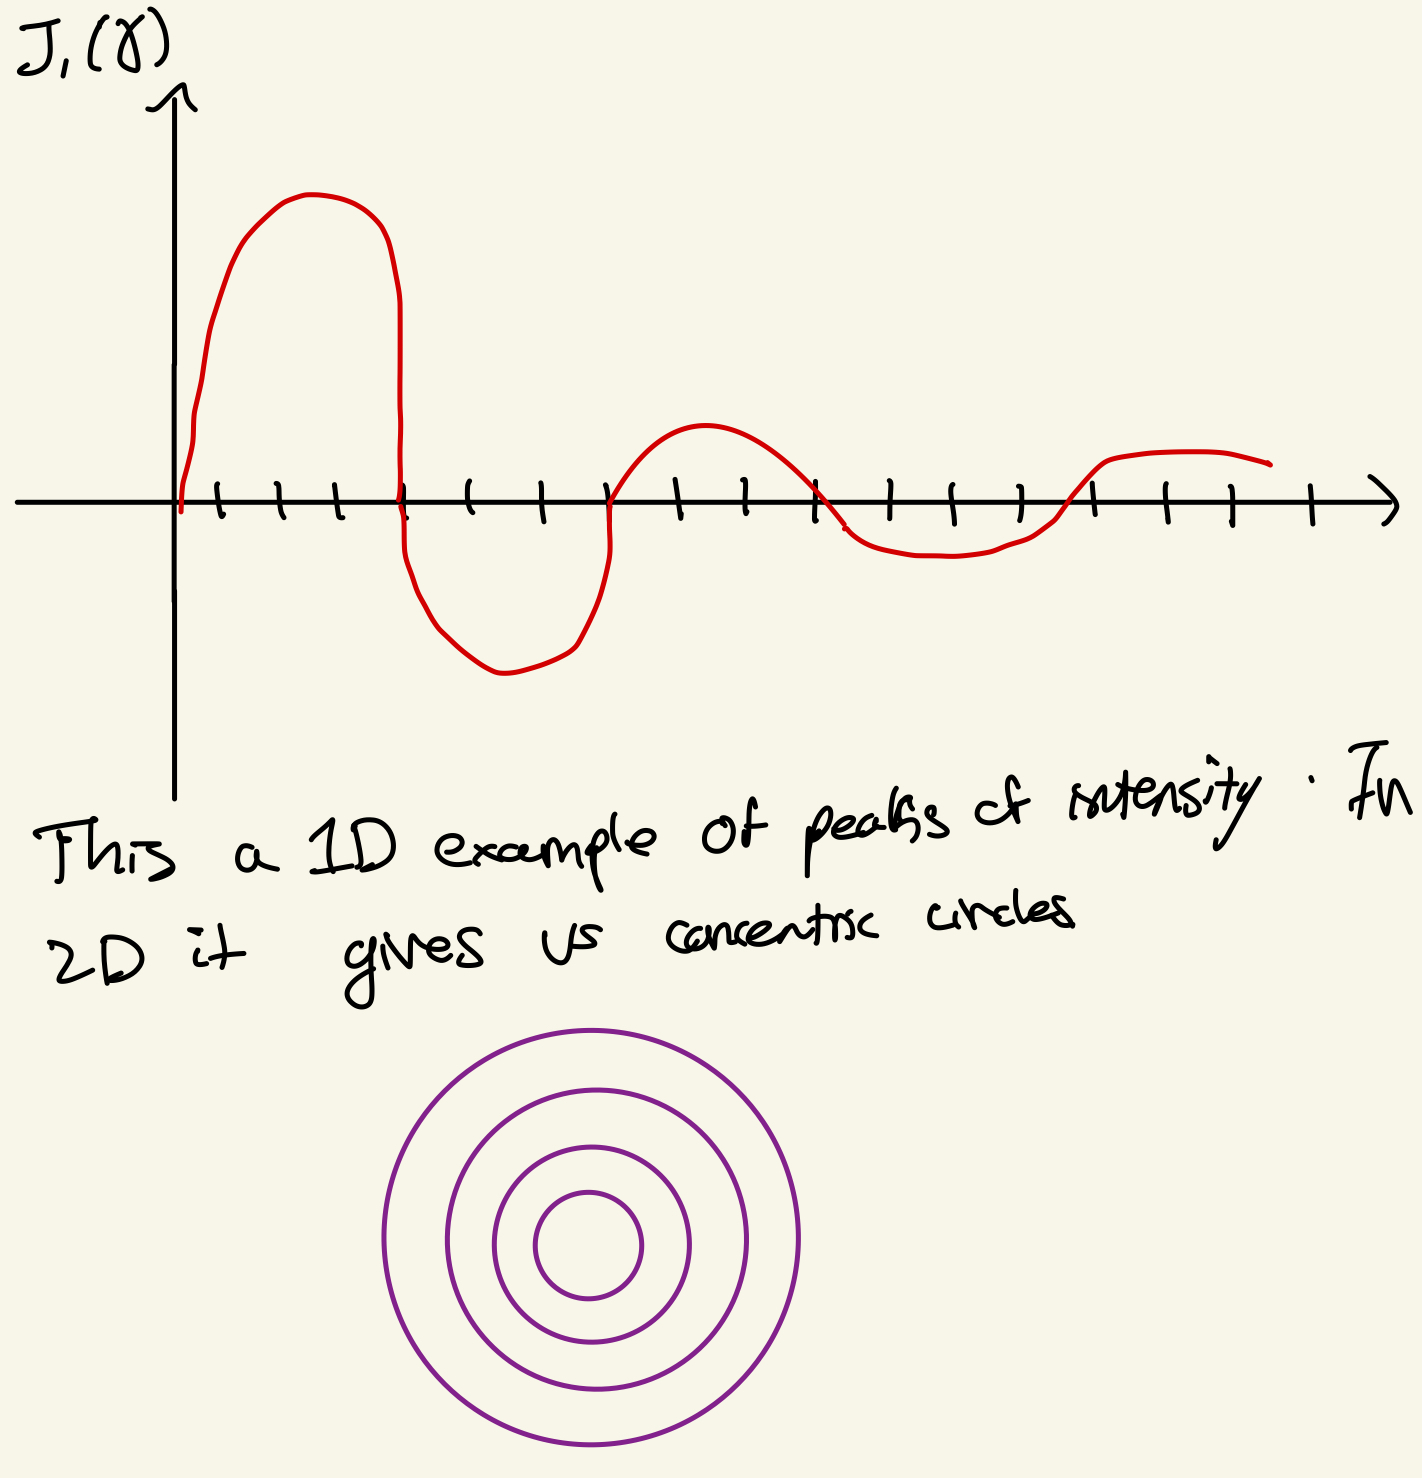
\includegraphics[scale = .2]{imgs/intesity-circ.jpeg}
\end{center}

and $J_1(\gamma)$ is the first-order Bessel function of the first kind.

\begin{center}
    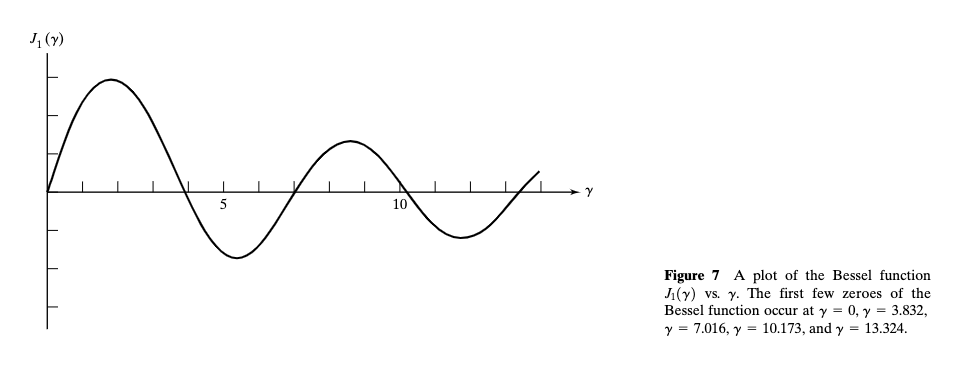
\includegraphics[scale = .8]{imgs/bessel-function.png}
\end{center}

\begin{center}
    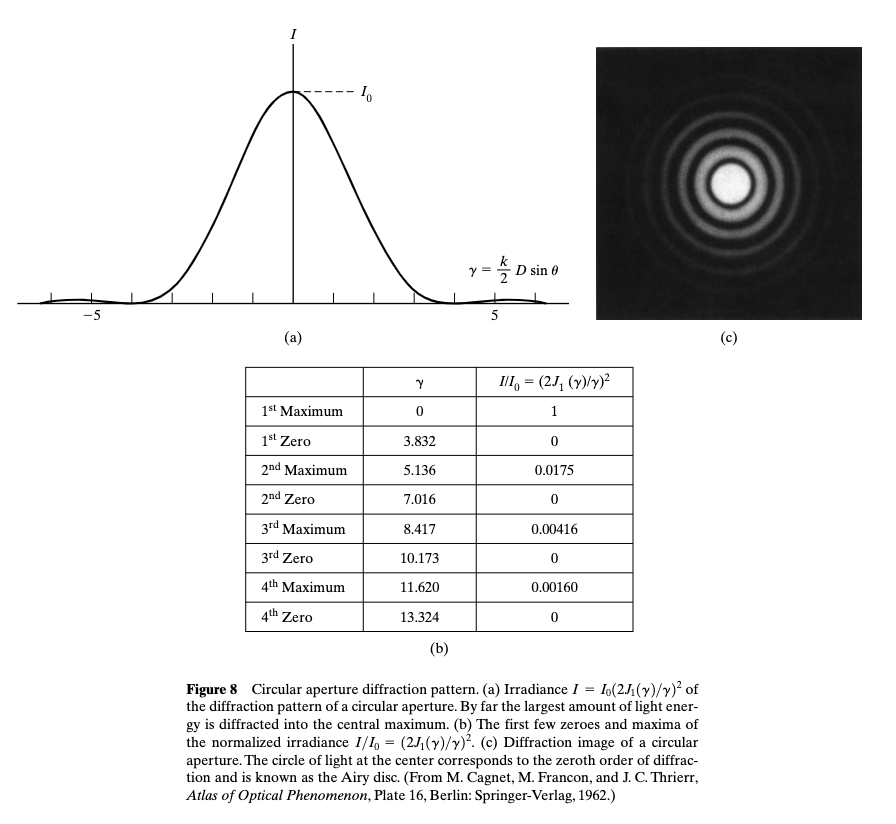
\includegraphics[scale = .7]{imgs/j.png}
\end{center}

\lo{Determine the resolution of imaging devices by means of Rayleigh’s criterion}

As shown above, the intensity for a circular aperture gives us

\begin{center}
    \includegraphics*[scale = .8]{imgs/intesity-from-circ-app.png}
\end{center}

The pattern in Figure 7 is symmertrical about the optical axis throught the center of the circular aperature and has its first zero when $\gamma = 3.828$ as shown in Figure 8a and b,therefore, the irradiance first falls to zero when 
\[Dsin(\theta) = 1.22 \lambda\]

\newpage

The idffracted image of a circular aperture forms and intensity patter called an Airy disc. The far-field angular ardius of the Airy pattern is 

\[\Delta \theta_{1/2} = \frac{1.22 \lambda}{D}\]

Let's saw we have two point objects $s_1$ and $s_2$ imaged by a lens, then the center of the two Airy discs are resolved by $\theta$. This leads us to \textbf{Rayleigh's criterion} which is defined as, for just resolvable images, the angular separation of the centers should be no less than the angular radius of the air disc which is given by 
\[(\Delta \theta) = \frac{1.22 \lambda}{D}\]

This is achievable by either using a shorter wavelength $\lambda$ or a higher diameter will give us reduced refraction.

\begin{center}
    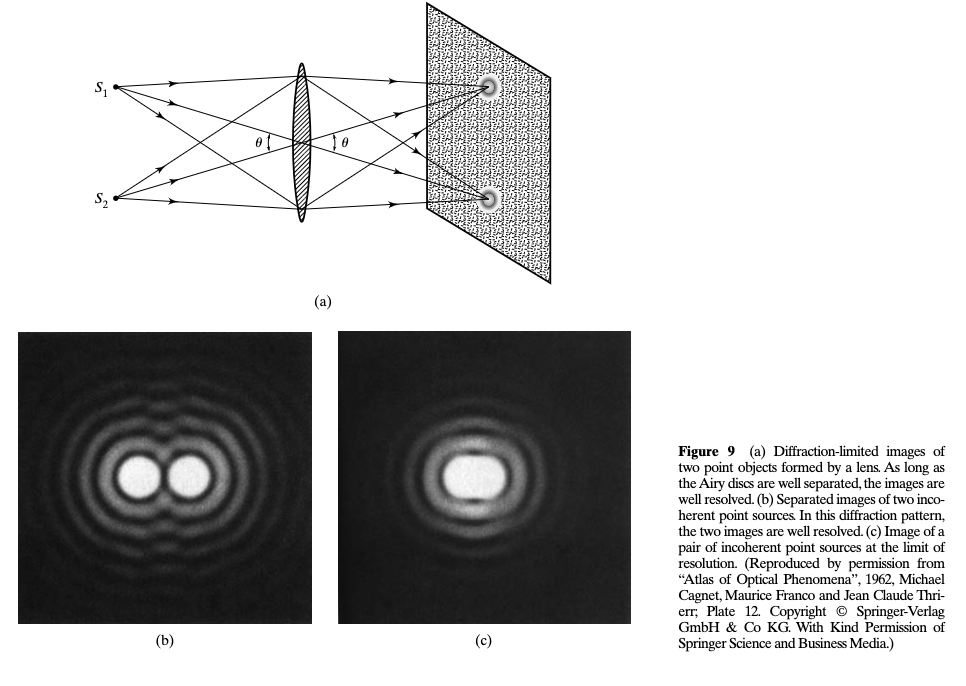
\includegraphics[scale = 1]{imgs/rayleigh.png}
    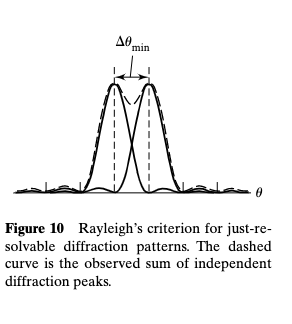
\includegraphics[scale = .9]{imgs/fig-10.png}
\end{center}

\newpage

\lo{Use the diffraction equation to determine the direction of principal diffraction maxima. Determine the free spectral range, the dispersion, and the resolution of a grating}

Lets say we want to we want to measure distances between these two bight spots, but they're smudgy (look at Airy function), so there a better way to make these constructive interference so we can measure them! We will make something with a ton of holes, and the screen or film will have dots instead of these Airy functions!

Let's see the diagram below:

\begin{center}
    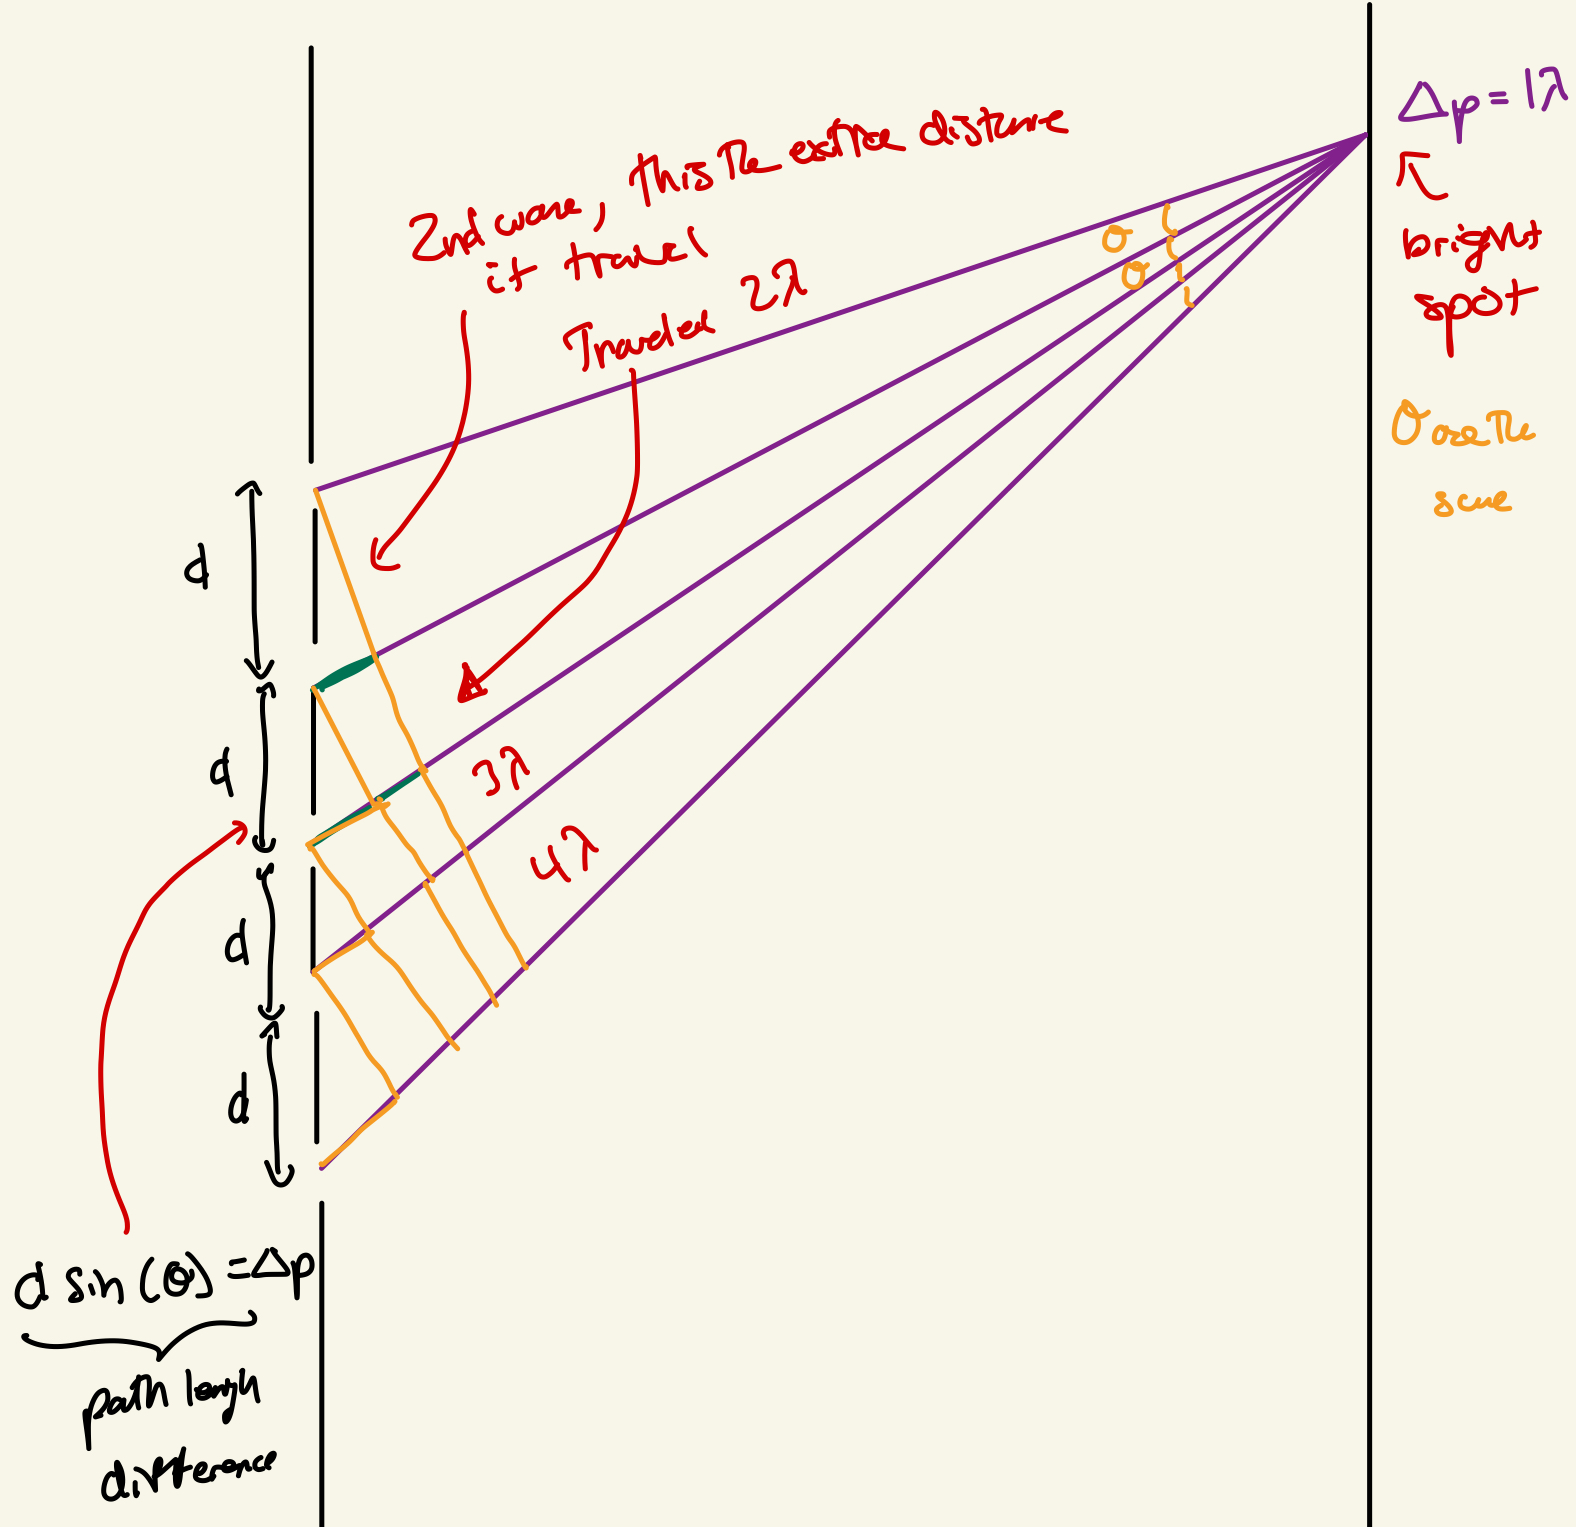
\includegraphics[scale = .2]{imgs/grating.jpeg}
\end{center}

We see if we have many slits that they will all have a constructive interference at one spot (remember that we have constructive interference when the peaks of the wave match the peaks, and troughs match the troughs). If we go slightly off, lets say 1.1 of a wavelength then there will be total destructive interference. So the screen will only show dots because of all the constructive interferences on the wall.

\newpage

Let's look at the diagram below:

\begin{center}
    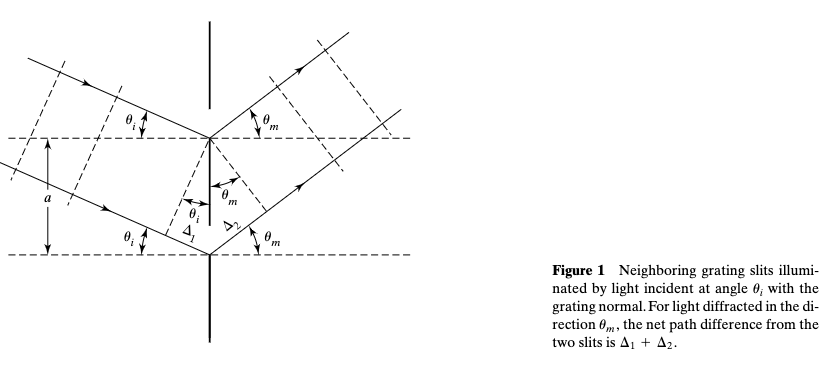
\includegraphics[scale = .7]{imgs/diffratction-fig-1.png}
\end{center}

The optical path difference for waves from successive slits is 

\[\Delta = \Delta 1 + \Delta 1 = a(\sin(\theta_i) + \sin(\theta_m))\]

Where we use the sign convention of 
\begin{itemize}
    \item + $\theta_m$ if on the same side of the normal as $\theta_i$
    \item - $\theta_m$ if on the opposite side of the normal as $\theta_i$
\end{itemize}

Constructive interference when $\Delta = m \lambda$, give us the \textbf{grating equation}

\[a(\sin(\theta_i) + \sin(\theta_m)) = m \lambda\]

If we have $\lambda_1$ be the shortest wavelength and $\lambda_2$ be the longest wavelength of the incident light that is non-overlapping with the next order $\lambda_1$, then 
\[m\lambda_2 = (m+1)\lambda_1\]
Therefore we can define the free-spectral range $\lambda_{fsr}$, the maximum wavelength separation thaat can be unambiguously resolve in a given order, 

\[\lambda_{fsr} = \lambda_2 - \lambda_1 = \frac{\lambda_1}{m}\]

The free spectral range is the maximum wavelength separation $\Delta \lambda_{max}$, that can be unambiguously solved in any given order.

\textbf{Dispersion of grating}

The grating is spreading out the different wavelengths















\end{document}